% !TEX root = ../main.tex
\chapter{Badania i analiza}
\label{chap:badania-i-analiza}

\section{Wybór benchmarków oraz metryk oceny jakości odpowiedzi}

\subsection{Benchmarki}
\label{sec:benchmarki}

Do badań wybrano dwa publicznie dostępne zbiory zadań, które stawiają modelom różne wymagania: MATH-500 sprawdza rozumowanie, a MedMCQA wiedzę. Dzięki temu można ustalić, czy debata pomaga niezależnie od rodzaju zadania, czy tylko w jednym z nich. Oba zbiory mają odpowiedź wzorcową, którą da się zweryfikować automatycznie, bez udziału człowieka ani modelu oceniającego.

\subsubsection{MATH-500}

Jest to podzbiór 500 zadań z benchmarku MATH \cite{hendrycksmath2021}, wybrany przez OpenAI na potrzeby pracy \emph{Let's Verify Step by Step} \cite{lightman2023verify}. Zadania pochodzą z konkursów matematycznych. Odpowiedź jest otwarta: model podaje liczbę lub wyrażenie, a nie wybiera spośród gotowych opcji, więc trafienie przypadkiem jest mało prawdopodobne. Rozwiązanie zwykle składa się z kilku kroków, które można sprawdzić po kolei. Taki charakter zadań sprzyja debacie, bo błąd w rozumowaniu jednego modelu może wskazać drugi.

\subsubsection{MedMCQA} 

Zbiór \cite{pmlr-v174-pal22a} zawiera ponad 194~tys. pytań z egzaminów wstępnych AIIMS i NEET~PG. Obejmuje 21 przedmiotów i około 2,4~tys. tematów medycznych. Każde pytanie ma cztery opcje odpowiedzi i dokładnie jedną poprawną. O wyniku decyduje przede wszystkim wiedza, a nie długie rozumowanie. MedMCQA jest więc przeciwieństwem MATH-500 i pozwala sprawdzić, czy debata pomaga także wtedy, gdy zadanie sprowadza się do przypomnienia faktu. Zamknięty format ma jedną konsekwencję: losowy wybór daje 25\% poprawnych odpowiedzi, co należy uwzględniać przy interpretacji wyników.

\subsubsection{Dobór zadań}

Do testu wybrano po 250 zadań z każdego zbioru. Zadania wybrano w orginalnej kolejności występowania w zbiorze, bez losowania. Ze zbioru \texttt{HuggingFaceH4/MATH-500} (split \texttt{test}) i \texttt{openlifescienceai/medmcqa} (split \texttt{validation}). Tak określony podzbiór jest stały, więc eksperyment można dokładnie powtórzyć. Wszystkie konfiguracje modeli rozwiązywały te same zadania, co umożliwia porównania parowane po identyfikatorze zadania (sekcja~\ref{sec:metryki}). Zestawienie zbiorów przedstawia tabela \ref{tab:zestawienie_benchmarkow}.

% !TEX root = ../main.tex
\begin{table}[H]
    \centering
    \caption{Zestawienie wykorzystanych benchmarków}
    \label{tab:zestawienie_benchmarkow}
    \begin{tabular}{|l|l|l|}
        \hline
        \rowcolor{gray!20}
        & \textbf{MATH-500} & \textbf{MedMCQA} \\ \hline
        Dziedzina & matematyka & medycyna \\ \hline
        Odpowiedź & otwarta & jedna z opcji A--D \\ \hline
        Co sprawdza & rozumowanie & wiedzę \\ \hline
        Źródło & konkursy matematyczne & egzaminy AIIMS i NEET PG \\ \hline
        Podzbiór & 250 pierwszych zadań, \texttt{test} & 250 pierwszych pytań, \texttt{validation} \\ \hline
    \end{tabular}
\end{table}

\subsection{Metryki oceny}
\label{sec:metryki}

\subsubsection{Ocena odpowiedzi}

Wynik zadania porównuje się z odpowiedzią wzorcową tą samą funkcją oceny w każdej konfiguracji, więc tryb pojedynczego modelu i tryb debaty są oceniane identycznie. W MATH-500 odpowiedzi poddaje się normalizacji według procedury Hendrycksa \cite{hendrycksmath2021}, a jeśli porównanie napisów nie wystarcza, sprawdza się równoważność symboliczną biblioteką \texttt{sympy}. Dzięki temu różne zapisy tej samej wartości, na przykład ułamek zwykły i jego postać w \LaTeX{}u, nie są uznawane za błąd. W MedMCQA porównuje się wskazaną literę z zakresu A--D. Ta sama funkcja równoważności służy w debacie do stwierdzenia, czy modele doszły do zgody.

\subsubsection{Kategorie wyniku}

Każde zadanie kończy się jednym z czterech wyników:
\begin{itemize}
    \item \emph{poprawny} -- odpowiedź zgodna z wzorcową,
    \item \emph{błędny} -- udzielona odpowiedź jest niezgodna z wzorcową,
    \item \emph{abstain} -- w debacie modele nie doszły do zgody po trzech rundach, więc system nie zwraca odpowiedzi,
    \item \emph{null} -- w trybie pojedynczego modelu generacja została ucięta po przekroczeniu limitu 6000 tokenów i nie zawiera odpowiedzi.
\end{itemize}

Taki podział pokazuje, w jaki sposób system zawodzi, czego nie widać w samym odsetku poprawnych odpowiedzi. Przyjęto hierarchię, w której poprawna odpowiedź jest najlepsza, a błędna najgorsza. Abstain uznano za lepszy od błędu i od null, ponieważ system, który nie ma pewności, powinien raczej powstrzymać się od odpowiedzi, niż halucynować.

\subsubsection{Dokładność}

Główną miarą jest dokładność, czyli odsetek zadań rozwiązanych poprawnie spośród wszystkich zebranych ($n = 250$). Abstain i null pozostają w mianowniku, więc dokładność nie zawyża wyniku systemu, który często rezygnuje z odpowiedzi. Uzupełnia ją rozkład czterech kategorii wyniku, a w szczególności odsetek odpowiedzi błędnych.

\subsubsection{Istotność statystyczna}

Wszystkie konfiguracje rozwiązywały te same zadania, więc różnice dokładności oceniono dokładnym testem McNemara \cite{mcnemar1947note}, który działa na parach wyników. Test uwzględnia tylko zadania, w których jedna z porównywanych konfiguracji odpowiedziała poprawnie, a druga nie. Przy $n$ takich zadaniach, z których $k$ rozwiązała tylko ta konfiguracja, która rozwiązała ich mniej, dwustronna wartość $p$ wynosi

\begin{equation}
    p = \min\!\left(1,\; 2 \cdot 2^{-n} \sum_{i=0}^{k} \binom{n}{i}\right).
\end{equation}

Przyjęto poziom istotności $\alpha = 0{,}05$. Wyniki zebrano w tabeli~\ref{tab:testy_parowane}.

\subsubsection{Metryki diagnostyczne debaty}

Sama dokładność nie wyjaśnia, jak debata zmienia wynik. Dlatego dla każdej debaty zestawiono wynik końcowy z rundą niezależną, w której modele odpowiadają, nie znając odpowiedzi drugiego. Na tej podstawie wyznaczono odsetek zadań rozstrzygniętych bez debaty oraz liczbę zadań uratowanych i utraconych. Definicje tych miar i ich interpretacja znajdują się w sekcji~\ref{sec:kiedy_debata_pomaga}.

\subsubsection{Koszt obliczeniowy}
\label{sec:koszt_metryka}

Koszt mierzono na jedno zadanie: liczbą tokenów (wejściowych i wygenerowanych, zliczonych we wszystkich wywołaniach modeli) oraz średnim czasem rozwiązania. Pomiary wykonano na tym samym komputerze, więc wartości dla debaty można bezpośrednio porównywać z wartościami dla pojedynczego modelu (sekcja~\ref{sec:koszt}).

\section{Przeprowadzenie analizy wyników oraz porównanie jakości odpowiedzi w obu trybach działania systemu}

Analizie poddano pięć konfiguracji systemu na dwóch zbiorach danych, MATH-500 i MedMCQA. W każdym rozwiązano po 250 identycznych zadań we wszystkich konfiguracjach modeli. Modele \texttt{qwen3.5:9b} i \texttt{gemma4:12b} oznaczono odpowiednio jako Q i G. Tryb pojedynczego modelu (solo) reprezentują Q i G, a tryb współpracy -- debaty jednorodne Q+Q i G+G oraz debata mieszana Q+G. Każdą konfigurację uruchomiono z ustalonym ziarnem. Różnice oceniono testem McNemara na odpowiadających sobie zadaniach. Analizę uporządkowano: kolejne podsekcje omawiają jakość odpowiedzi, warunki, w których debata pomaga, koszt obliczeniowy oraz niepowodzenia generacji.

\subsection{Jakość odpowiedzi}
\label{sec:jakosc}

Główną miarą jakości jest dokładność, czyli odsetek zadań rozwiązanych poprawnie spośród wszystkich zebranych. Nie oznacza to, że pozostałe wyniki są równoważne: abstain, czyli brak konsensusu w debacie, uznano za lepszy od odpowiedzi błędnej i od null, ponieważ system, który nie ma pewności, powinien raczej powstrzymać się od odpowiedzi, niż halucynować. Z tego względu tabela~\ref{tab:wyniki_zbiorcze} i wykres~\ref{wyk:sklad_wynikow} pokazują rozkład czterech kategorii wyników, a nie tylko odsetek poprawnych.

% !TEX root = ../main.tex
\begin{table}[H]
    \centering
    \caption{Wyniki zbiorcze dla obu zbiorów danych ($n = 250$ zadań na zbiór)}
    \label{tab:wyniki_zbiorcze}
    \small
    \setlength{\tabcolsep}{2.5pt}
    \renewcommand{\arraystretch}{1.35}
    \sbox0{%
    \begin{tabular}{|>{\centering\arraybackslash}p{2.0cm}|>{\centering\arraybackslash}p{2.2cm}|>{\centering\arraybackslash}p{1.7cm}|>{\centering\arraybackslash}p{1.45cm}|>{\centering\arraybackslash}p{1.55cm}|>{\centering\arraybackslash}p{1.25cm}|>{\centering\arraybackslash}p{1.7cm}|>{\centering\arraybackslash}p{2.0cm}|}
        \hline
        \rowcolor{gray!20}
        \multicolumn{2}{|c|}{} & \multicolumn{4}{c|}{\textbf{Odsetek zadań [\%]}} & \textbf{Średni} & \textbf{Tokeny} \\ \cline{3-6}
        \rowcolor{gray!20}
        \textbf{Zbiór} & \textbf{Konfiguracja} & \textbf{Poprawne} & \textbf{Błędne} & \textbf{Abstain} & \textbf{Null} & \textbf{czas [s]} & \textbf{na zadanie} \\ \hline
        Matematyka & Q & 60,8 & 35,6 & -- & 3,6 & 13,5 & 760 \\ \cline{2-8}
         & G & 78,0 & 13,2 & -- & 8,8 & 27,8 & 955 \\ \cline{2-8}
         & Q+Q & 72,0 & 26,0 & 2,0 & -- & 52,9 & 3\,291 \\ \cline{2-8}
         & Q+G & \textbf{85,6} & 8,8 & 5,6 & -- & 103,7 & 4\,525 \\ \cline{2-8}
         & G+G & 81,2 & 12,4 & 6,4 & -- & 125,2 & 4\,128 \\ \hline
        Medycyna & Q & 66,4 & 32,8 & -- & 0,8 & 7,8 & 508 \\ \cline{2-8}
         & G & 60,4 & 38,4 & -- & 1,2 & 8,5 & 440 \\ \cline{2-8}
         & Q+Q & \textbf{70,0} & 27,2 & 2,8 & -- & 19,7 & 1\,575 \\ \cline{2-8}
         & Q+G & 68,0 & 27,6 & 4,4 & -- & 34,8 & 2\,145 \\ \cline{2-8}
         & G+G & 62,4 & 37,6 & 0,0 & -- & 16,2 & 1\,042 \\ \hline
    \end{tabular}}
    \usebox{0}
    \par\smallskip
    \begin{minipage}{\wd0}
        \raggedright\footnotesize
        Q -- \texttt{qwen3.5:9b}, G -- \texttt{gemma4:12b}; Q+Q, Q+G i G+G -- debata odpowiednich par modeli. Czas i liczba tokenów dotyczą jednego zadania, a tokeny (wejściowe i wygenerowane) zliczono we wszystkich wywołaniach modeli. Pogrubiono najwyższy odsetek poprawnych odpowiedzi w zbiorze.
    \end{minipage}
\end{table}


Rozpiętość wyników zależy od zbioru. W matematyce dokładność waha się od 60,8\% (Q) do 85,6\% (Q+G), czyli o 24,8 punktu procentowego (pp), a w medycynie od 60,4\% (G) do 70,0\% (Q+Q), czyli o 9,6~pp. Zbiór matematyczny pokazuje wyraźne różnice między konfiguracjami, natomiast w medycynie wszystkie leżą blisko siebie.

\begin{wykres}[H]
    \centering
    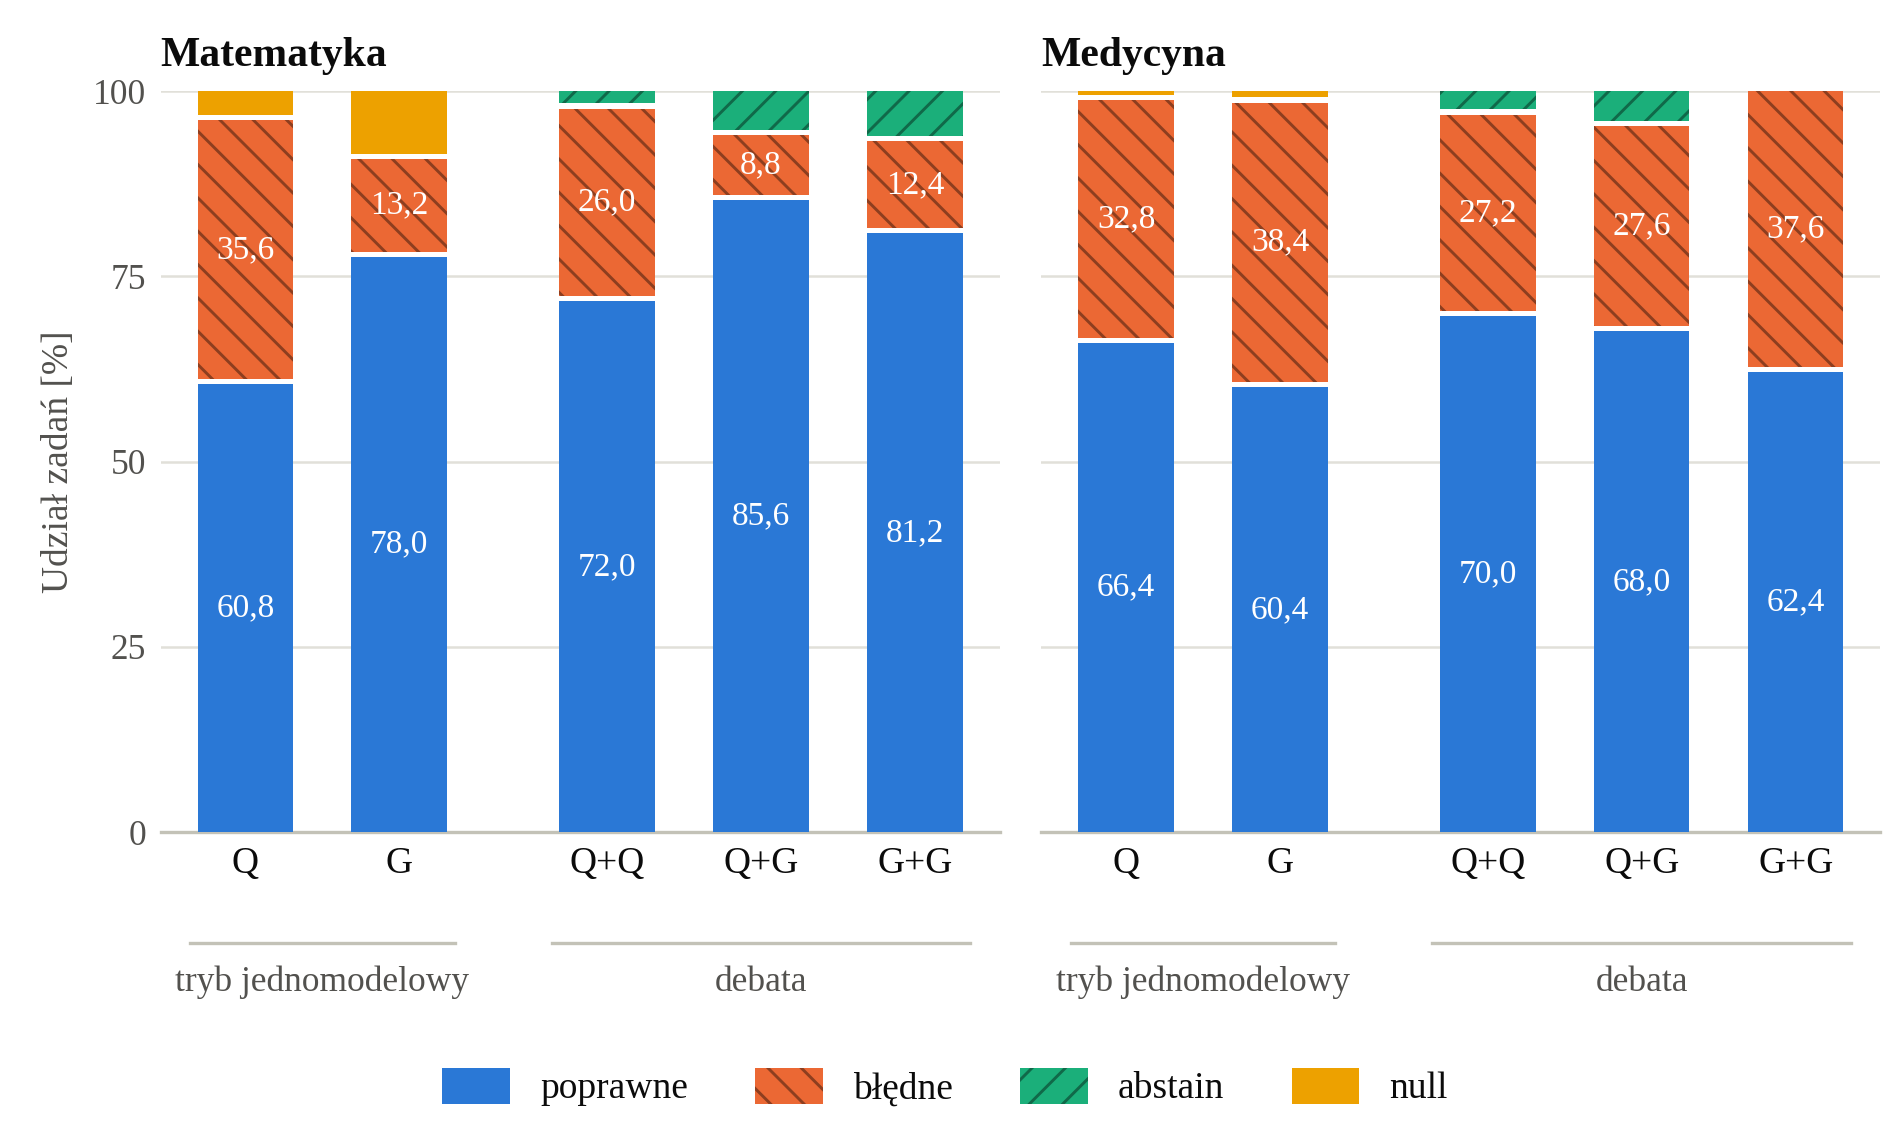
\includegraphics[width=\textwidth]{figures/rys-sklad-wynikow.png}
    \caption{Skład wyników w poszczególnych konfiguracjach: odsetek zadań poprawnych, błędnych, abstain i null ($n = 250$ zadań na zbiór)}
    \label{wyk:sklad_wynikow}
\end{wykres}

W matematyce G przewyższa Q o 17,2~pp ($p < 0{,}001$), chociaż 8,8\% zadań kończy się u niego wynikiem null, czyli generacją uciętą po wyczerpaniu okna kontekstu o długości 4096 tokenów (sekcja~\ref{sec:niepowodzenia}). Przewagę zawdzięcza małemu udziałowi odpowiedzi błędnych: 13,2\% wobec 35,6\% w Q. W medycynie kolejność jest odwrotna: Q jest lepszy o 6,0~pp (66,4\% wobec 60,4\%). Można przypuszczać, że modele mają mocne i słabe strony, na przykład G lepiej radzi sobie z rozumowaniem wieloetapowym, a Q z zadaniami wiedzowymi, jednak przeprowadzone eksperymenty tego jednoznacznie nie rozstrzygają.

% !TEX root = ../main.tex
\begin{table}[H]
    \centering
    \caption{Porównania parami konfiguracji na tych samych zadaniach}
    \label{tab:testy_parowane}
    \small
    \setlength{\tabcolsep}{2.5pt}
    \renewcommand{\arraystretch}{1.35}
    \sbox0{%
    \begin{tabular}{|>{\centering\arraybackslash}p{3.2cm}|>{\centering\arraybackslash}p{1.3cm}|>{\centering\arraybackslash}p{1.35cm}|>{\centering\arraybackslash}p{1.35cm}|>{\centering\arraybackslash}p{1.4cm}|>{\centering\arraybackslash}p{1.3cm}|>{\centering\arraybackslash}p{1.35cm}|>{\centering\arraybackslash}p{1.35cm}|>{\centering\arraybackslash}p{1.4cm}|}
        \hline
        \rowcolor{gray!20}
        \multicolumn{1}{|c|}{} & \multicolumn{4}{c|}{\textbf{Matematyka}} & \multicolumn{4}{c|}{\textbf{Medycyna}} \\ \cline{2-9}
        \rowcolor{gray!20}
        \textbf{Porównanie} & \textbf{$\Delta$ [pp]} & \textbf{tylko A} & \textbf{tylko B} & \textbf{p} & \textbf{$\Delta$ [pp]} & \textbf{tylko A} & \textbf{tylko B} & \textbf{p} \\ \hline
        Q+Q vs Q & $+$11,2 & 33 & 5 & \textbf{$<$0,001} & $+$3,6 & 13 & 4 & \textbf{0,049} \\ \hline
        G+G vs G & $+$3,2 & 11 & 3 & 0,057 & $+$2,0 & 10 & 5 & 0,302 \\ \hline
        Q+G vs lepszy solo & $+$7,6 & 22 & 3 & \textbf{$<$0,001} & $+$1,6 & 21 & 17 & 0,627 \\ \hline
        Q+G vs Q+Q & $+$13,6 & 43 & 9 & \textbf{$<$0,001} & $-$2,0 & 13 & 18 & 0,473 \\ \hline
        Q+G vs G+G & $+$4,4 & 17 & 6 & \textbf{0,035} & $+$5,6 & 29 & 15 & \textbf{0,049} \\ \hline
        G vs Q & $+$17,2 & 58 & 15 & \textbf{$<$0,001} & $-$6,0 & 25 & 40 & 0,082 \\ \hline
    \end{tabular}}
    \usebox{0}
    \par\smallskip
    \begin{minipage}{\wd0}
        \raggedright\footnotesize
        A i B -- pierwsza i druga konfiguracja w wierszu; $\Delta$ -- różnica odsetka poprawnych odpowiedzi A $-$ B w punktach procentowych (pp); „tylko A” i „tylko B” -- liczba zadań rozwiązanych poprawnie wyłącznie przez daną konfigurację; p -- wartość p dokładnego testu McNemara, pogrubiona dla $p < 0{,}05$. Lepszy solo: G w matematyce, Q w medycynie.
    \end{minipage}
\end{table}


Debata zmniejsza odsetek odpowiedzi błędnych. We wszystkich ośmiu porównaniach debaty z jej modelami składowymi (Q+Q z Q, G+G z G oraz Q+G z Q i z G, w obu zbiorach) udział błędnych był niższy, choć skala spadku była bardzo zróżnicowana. Q+Q zmniejsza go o 9,6~pp w matematyce i 5,6~pp w medycynie, Q+G względem modelu solo o mniejszym odsetku błędnych (G w matematyce, Q w medycynie) odpowiednio o 4,4 i 5,2~pp, a G+G zaledwie o 0,8~pp w obu zbiorach. O tym, czy spadek błędnych przekłada się na dokładność, decyduje zbiór. W matematyce Q+Q zyskuje 11,2~pp względem Q, a więc więcej niż wynosi spadek liczby błędnych, ponieważ maleje też udział zadań bez odpowiedzi (z 3,6\% null do 2,0\% abstain). W medycynie spadek odsetka błędnych w Q+G względem Q (5,2~pp) daje wzrost poprawnych tylko o 1,6~pp, a pozostałe 3,6~pp przechodzi w abstain (z 0,8\% null do 4,4\%). Przy przyjętej hierarchii wyników także jest to zyskiem: system rzadziej odpowiada błędnie, a częściej zgłasza brak zgody między modelami.

Debata mieszana Q+G jest najlepszą konfiguracją w matematyce: przewyższa G o 7,6~pp, Q+Q o 13,6~pp oraz G+G o 4,4~pp i ma najmniejszy odsetek błędnych (8,8\%). W medycynie jej wynik (68,0\%) jest wyższy niż Q (o 1,6~pp) i G+G (o 5,6~pp) oraz niższy niż Q+Q (o 2,0~pp). Żaden z testów nie wskazuje konfiguracji znacząco lepszej od Q+G. W obu zbiorach Q+G nie ustępuje więc najlepszemu modelowi solo, a w matematyce jest od niego istotnie lepsza. Nie wymaga przy tym wcześniejszego rozpoznania, który model pasuje do dziedziny, a zachowuje tę pozycję mimo udziału słabszego z dwóch modeli (Q w matematyce, G w medycynie). W tym sensie debata mieszana jest w obu badanych zbiorach rozwiązaniem najbardziej uniwersalnym, choć kosztem największego zużycia tokenów (sekcja~\ref{sec:koszt}).

\subsection{Kiedy debata pomaga}
\label{sec:kiedy_debata_pomaga}

Aby ustalić skąd w debacie biorą się zmiany wyniku, każde zadanie porównano z rundą niezależną, w której modele odpowiadają nie znając odpowiedzi drugiego. Tabela~\ref{tab:bilans_debaty} dzieli zadania na trzy rozłączne grupy: takie, w których modele zgodziły się od razu, a debata się nie odbyła, oraz dwie grupy zadań poddanych debacie: takie, w których w rundzie niezależnej żaden model nie podał poprawnej odpowiedzi, i takie, w których poprawną odpowiedź podał jeden z modeli. Gdy nie podał jej żaden, poprawny wynik końcowy oznacza zadanie uratowane, ponieważ debata musiała wytworzyć odpowiedź, której nikt wcześniej nie miał. Gdy podał ją jeden z modeli, debata powinna ją zachować, a wynik końcowy, który nie jest poprawny, oznacza zadanie utracone.

% !TEX root = ../main.tex
\begin{table}[H]
    \centering
    \caption{Bilans debaty względem rundy niezależnej (liczba zadań, dla każdej debaty $n = 250$)}
    \label{tab:bilans_debaty}
    \small
    \setlength{\tabcolsep}{2.5pt}
    \renewcommand{\arraystretch}{1.35}
    \sbox0{%
    \begin{tabular}{|>{\centering\arraybackslash}p{2.0cm}|>{\centering\arraybackslash}p{1.4cm}|>{\centering\arraybackslash}p{1.3cm}|>{\centering\arraybackslash}p{1.9cm}|>{\centering\arraybackslash}p{1.3cm}|>{\centering\arraybackslash}p{1.9cm}|>{\centering\arraybackslash}p{1.3cm}|>{\centering\arraybackslash}p{1.9cm}|}
        \hline
        \rowcolor{gray!20}
        \multicolumn{2}{|c|}{} & \multicolumn{2}{c|}{\shortstack{\textbf{Zgoda}\\\textbf{od razu}}} & \multicolumn{2}{c|}{\shortstack{\textbf{Żaden model}\\\textbf{poprawny}}} & \multicolumn{2}{c|}{\shortstack{\textbf{Jeden model}\\\textbf{poprawny}}} \\ \cline{3-8}
        \rowcolor{gray!20}
        \textbf{Zbiór} & \textbf{Debata} & \textbf{razem} & \textbf{w tym poprawna} & \textbf{razem} & \textbf{w tym uratowane} & \textbf{razem} & \textbf{w tym utracone} \\ \hline
        Matematyka & Q+Q & 185 & 134 & 37 & 19 & 28 & 1 \\ \cline{2-8}
         & Q+G & 141 & 132 & 36 & 10 & 73 & 1 \\ \cline{2-8}
         & G+G & 207 & 185 & 30 & 8 & 13 & 3 \\ \hline
        Medycyna & Q+Q & 220 & 163 & 7 & 0 & 23 & 11 \\ \cline{2-8}
         & Q+G & 160 & 129 & 16 & 1 & 74 & 34 \\ \cline{2-8}
         & G+G & 229 & 150 & 10 & 1 & 11 & 6 \\ \hline
    \end{tabular}}
    \usebox{0}
    \par\smallskip
    \begin{minipage}{\wd0}
        \raggedright\footnotesize
        Zgoda od razu -- zadania, w których oba modele podały równoważne odpowiedzi w rundzie niezależnej, przed debatą; „w tym poprawna” -- gdy ta odpowiedź jest poprawna. Pozostałe zadania trafiły do debaty. Żaden model poprawny i Jeden model poprawny -- zadania z debatą, w których w rundzie niezależnej poprawną odpowiedź podał odpowiednio żaden albo jeden z modeli. Uratowane -- zadania z pierwszej z tych grup, w których wynik końcowy jest poprawny. Utracone -- zadania z drugiej, w których wynik końcowy nie jest poprawny, także gdy debata zakończyła się abstain.
    \end{minipage}
\end{table}


W matematyce debata działa w sposób naprawczy. We wszystkich trzech konfiguracjach debaty łącznie uratowano 37 ze 103 zadań, w których nikt nie miał poprawnej odpowiedzi w rundzie niezależnej. Spośród 114 zadań, w których poprawną odpowiedź w rundzie niezależnej miał jeden z modeli, poprawny wynik przetrwał w 96\% przypadków, a utracono 5. W medycynie jest odwrotnie: uratowano zaledwie 2 z 33 zadań, w których nikt nie miał poprawnej odpowiedzi w rundzie niezależnej. Z kolei spośród 108 zadań, w których ktoś ją miał, poprawny wynik przetrwał tylko w 53\% (57 zadań), a utracono 51 (w 13 utraconych debata skończyła się abstain). Utracone zadania mierzą skuteczność wyboru między odpowiedziami z rundy niezależnej, a nie stratę względem modelu solo, dlatego nie przeczą wynikowi z tabeli~\ref{tab:testy_parowane}, według którego debata w medycynie nie pogarsza dokładności. Można przypuszczać, że w matematyce poprawny tok rozumowania da się sprawdzić krok po kroku, więc argument modelu mającego rację ma szansę przekonać drugi, natomiast w MedMCQA odpowiedź zależy głównie od wiedzy, której debata nie uzupełni. Eksperymenty tego jednak nie rozstrzygają.

W większości zadań wynik ustala się jeszcze przed debatą: modele zgadzają się od razu w matematyce w 185 (Q+Q), 141 (Q+G) i 207 (G+G) zadaniach z 250, a w medycynie odpowiednio w 220, 160 i 229. Wiarygodność zgody zależy od składu pary. Dwa egzemplarze tego samego modelu częściej zgadzają się na odpowiedź błędną: w matematyce w 51 (Q+Q), 9 (Q+G) i 22 (G+G) zadaniach, a w medycynie odpowiednio w 57, 31 i 79. Wśród odpowiedzi uzgodnionych od razu, w debacie mieszanej poprawnych jest 94\% w matematyce i 81\% w medycynie, a w debatach jednorodnych 72\% (Q+Q) i 89\% (G+G) w matematyce oraz 74\% i 66\% w medycynie. Można przypuszczać, że błędy dwóch instancji jednego modelu są silniej skorelowane niż błędy dwóch różnych modeli.

Para mieszana częściej wchodzi w debatę: w matematyce w 109 zadaniach wobec 65 (Q+Q) i 43 (G+G), w medycynie w 90 wobec 30 i 21. O skutku decyduje zbiór. W matematyce poprawna odpowiedź przetrwała debatę prawie za każdym razem (Q+G: 72 z 73), a debata uratowała ponadto 10 zadań. Z tego względu większa liczba debat przekłada się tu na najlepszy wynik. W medycynie poprawna odpowiedź przetrwała debatę w obu parach w około połowie zadań (Q+Q: 12 z 23, Q+G: 40 z 74), w sytuacji gdy ktoś ją miał w rundzie niezależnej. Q+G utraciła więc więcej zadań (34 wobec 11 w Q+Q) głównie dlatego, że częściej debatowała. Te straty w przybliżeniu równoważą zysk z rzadszych zgodnych błędów (31 wobec 57 w Q+Q) i mogą tłumaczyć, dlaczego Q+G nie wyprzedza tam Q+Q. Większa liczba rund debaty jest też źródłem wyższego kosztu pary mieszanej (sekcja~\ref{sec:koszt}).

Abstain nie jest przypadkowy. Zadania, w których debata kończy się brakiem konsensusu, są trudne także dla pojedynczego modelu: odpowiedni model solo (Q dla Q+Q, G dla G+G, a dla Q+G lepszy z dwóch w danym zbiorze) rozwiązał poprawnie 5 z 35 takich zadań w matematyce (14\%) i 5 z 18 w medycynie (28\%). Abstain trafia więc głównie w zadania, z którymi pojedynczy model sobie nie radzi.

\subsection{Koszt}
\label{sec:koszt}

Koszt obliczeniowy rośnie wraz z liczbą modeli i rund. Koszt mierzono liczbą tokenów (prompt i generowana odpowiedź łącznie) oraz czasem rozwiązania zadania, uśrednionymi po wszystkich 250 zadaniach zbioru. W obu zbiorach debata zużywa od 2,4 do 4,7 razy więcej tokenów i od 1,9 do 4,5 razy więcej czasu niż odpowiadający jej model solo (dla debaty mieszanej przyjęto lepszy z dwóch modeli z tabeli~\ref{tab:wyniki_zbiorcze}). Konfiguracja mieszana zużywa najwięcej tokenów w obu zbiorach: 4,7 razy więcej niż G w matematyce i 4,2 razy więcej niż Q w medycynie, przy czasie dłuższym odpowiednio 3,7 i 4,5 razy. W matematyce najdłużej trwa jednak G+G (średnio 125,2~s na zadanie wobec 103,7~s dla Q+G).

Czy ten koszt się zwraca, zależy od zbioru (wykres~\ref{wyk:dokladnosc_koszt}). W matematyce G jest dokładniejszy od Q+Q (78,0\% wobec 72,0\%), choć zużywa 3,4 razy mniej tokenów. Dopiero G+G i Q+G przewyższają go dokładnością, ale przy 4,3 i 4,7 razy większych kosztach. Z kolei tylko zysk Q+G (7,6~pp, $p < 0{,}001$) jest istotny, a zysk G+G (3,2~pp, $p = 0{,}057$) tej istotności nie osiąga. W medycynie Q+Q poprawia wynik Q o 3,6~pp ($p = 0{,}049$) przy 3,1 razy większym koszcie, a Q+G zużywa 1,4 razy więcej tokenów niż Q+Q i nie ustępuje istotnie dokładnością (68,0\% wobec 70,0\%). Większy koszt debaty wyraźnie zwraca się więc tylko w matematyce.

\begin{wykres}[H]
    \centering
    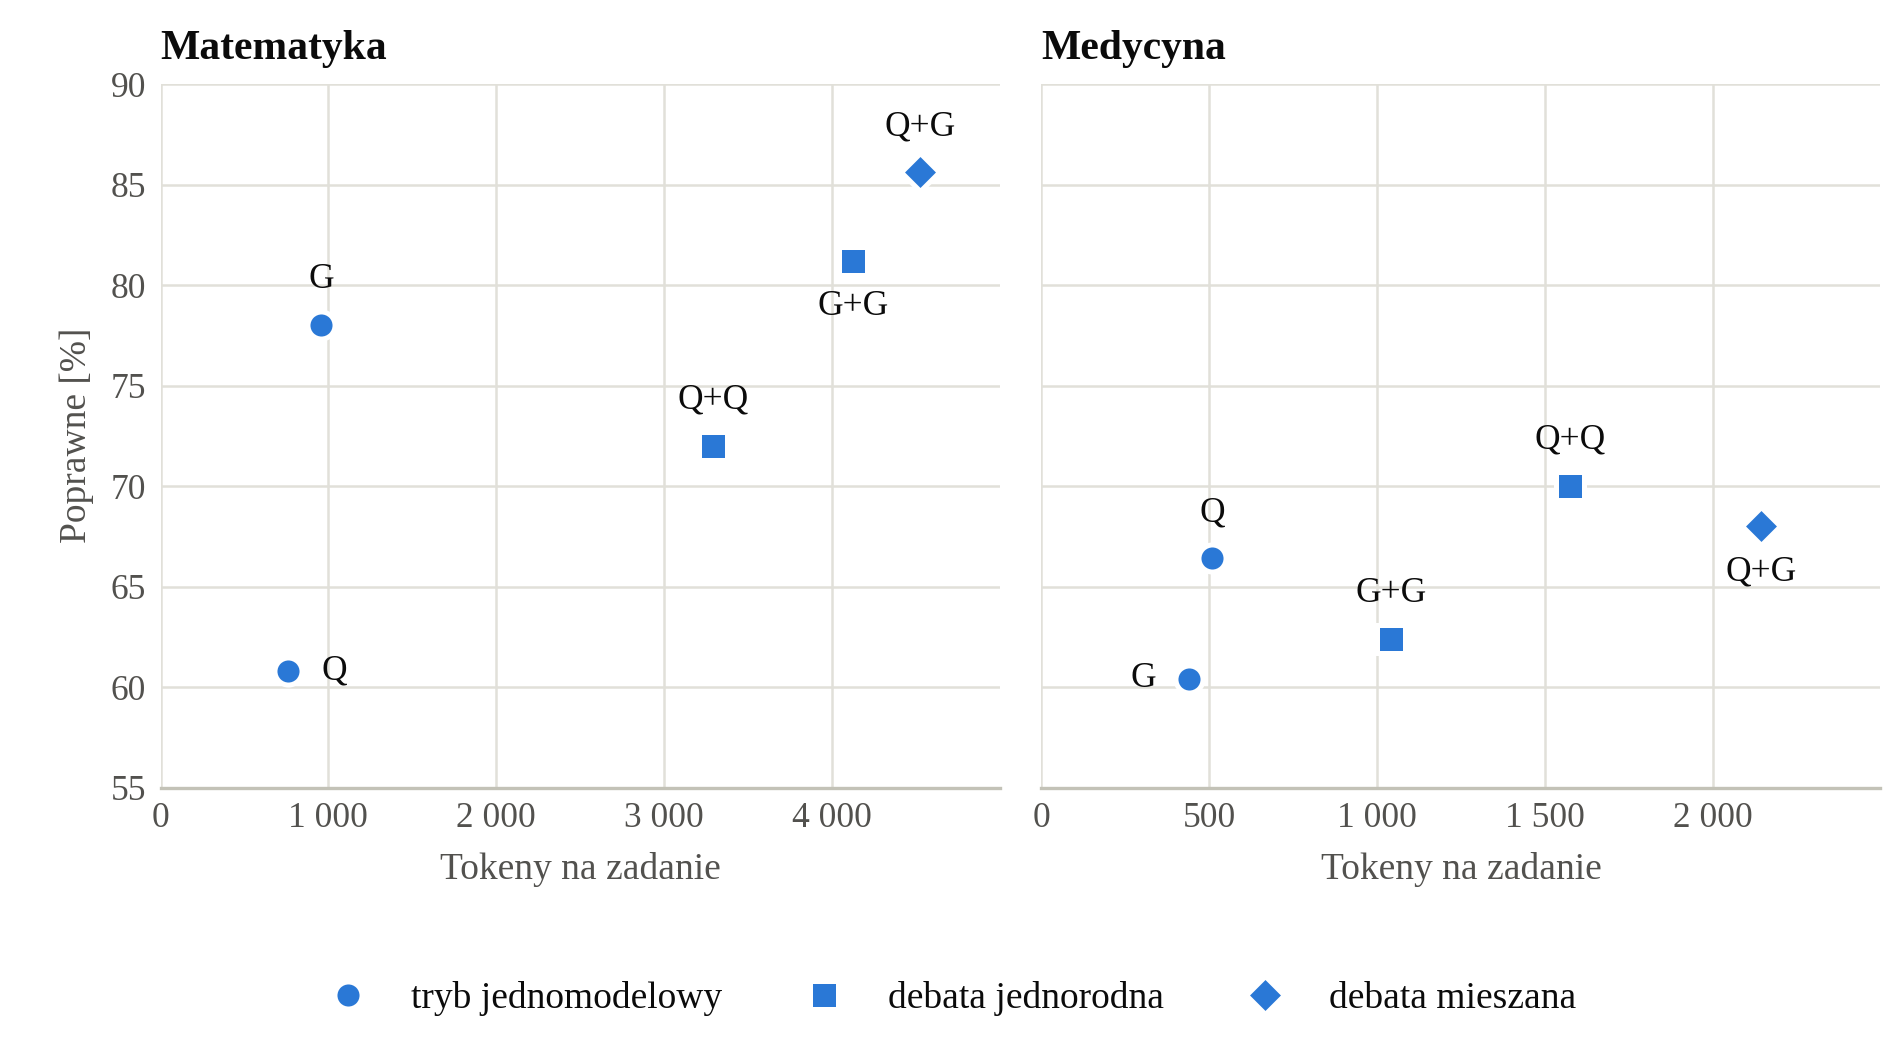
\includegraphics[width=\textwidth]{figures/rys-dokladnosc-koszt.png}
    \caption{Dokładność a liczba tokenów na zadanie w poszczególnych konfiguracjach}
    \label{wyk:dokladnosc_koszt}
\end{wykres}

Koszt debaty składa się z rundy niezależnej, w której oba modele odpowiadają jak w trybie solo, oraz z rund debaty. Runda niezależna zużywa 1,6--2,0~tys.~tokenów na zadanie w matematyce i 0,8--1,0~tys.\ w medycynie, czyli w przybliżeniu sumę kosztów obu modeli w trybie solo. Rundy debaty odpowiadają za od 21\% (G+G w medycynie) do 62\% (Q+G w matematyce) wszystkich tokenów i za 17--54\% czasu.

W matematyce kolejne rundy nie są tańsze od pierwszej. W Q+G jedna runda kosztuje w matematyce średnio 3,8~tys.~tokenów i 65~s w rundzie 1 oraz 5,2~tys.~tokenów i 118--126~s w rundach 2 i 3, ponieważ odpowiedzi modeli są w rundach 2 i 3 około dwa razy dłuższe niż w rundzie 1, a prompt, około czterokrotnie dłuższy niż w rundzie niezależnej, od rundy 1 już nie rośnie. W medycynie koszt rundy jest podobny w każdej z trzech (2,1--2,3~tys.~tokenów, 25--30~s). W Q+G odsetek poprawnych wyników wśród zadań, które kończą się w danej rundzie, spada w matematyce z 89\% w rundzie 1 do 70\% w rundzie 2 i 30\% w rundzie 3, a w medycynie z 60\% do 25\% i 18\%. Co najmniej połowa zadań, które doszły do rundy 3, kończy się abstain, a sama runda 3 zużywa 6--12\% wszystkich tokenów debaty (G+G w medycynie w ogóle do niej nie dochodzi). Z uwagi na to, wydłużanie debaty ponad przyjęte trzy rundy byłoby mało opłacalne.

W obu zbiorach dokładniejszy jest model zużywający więcej tokenów: w matematyce G (955 tokenów na zadanie wobec 760 dla Q), w medycynie Q (508 wobec 440). W debacie mieszanej wzorzec się powtarza (matematyka: G 2,4~tys.~tokenów wobec 2,1~tys.\ dla Q; medycyna: Q 1,2~tys.\ wobec 1,0~tys.). Znaczną część kosztu stanowią wywołania ucięte po wyczerpaniu okna kontekstu (sekcja~\ref{sec:niepowodzenia}): w trybie solo 22 ucięte generacje G w matematyce zużywają 38\% tokenów, jakie G zużył na wszystkie 250 zadań tego zbioru, a w debatach w matematyce takie wywołania stanowią 24\% wszystkich tokenów w Q+Q, 37\% w Q+G i 57\% w G+G. W debatach w medycynie stanowią nie więcej niż 5,2\%.

\subsection{Niepowodzenia generacji i tryb rozumowania}
\label{sec:niepowodzenia}

Wynik null w trybie solo oznacza generację uciętą po wyczerpaniu okna kontekstu o długości 4096 tokenów, które obejmuje zarówno prompt, jak i generowany tekst. Takich wyników jest 36 na 1000 zadań rozwiązanych w trybie solo. Dotyczą głównie matematyki: rezultat null ma 3,6\% zadań Q i 8,8\% zadań G wobec 0,8\% i 1,2\% w medycynie, co zgadza się z tym, że odpowiedzi na zadania matematyczne są dłuższe (średnio 760 i 955 tokenów per zadanie wobec 508 i 440 w medycynie).

Debata nie zwraca wyniku null, ponieważ ucięta generacja oznacza w niej brak odpowiedzi jednego z modeli, a nie koniec zadania. Konsensus wymaga odpowiedzi od wszystkich modeli, więc debata przechodzi do kolejnej rundy, a po trzeciej kończy się abstain. W debatach matematycznych ucięcia są częstsze niż w trybie solo: dotyczą 6,9\% wywołań w Q+Q, 12,2\% w Q+G i 21,5\% w G+G wobec 3,6\% Q i 8,8\% G w trybie solo. Z kolei w medycynie stanowią 0,4--0,8\% wywołań. Zdarzają się też częściej w rundach debaty niż w rundzie niezależnej (w matematyce: w Q+Q 14,8\% wobec 3,8\%, w Q+G 20,9\% wobec 6,4\%, w G+G 55,3\% wobec 10,0\%). Prompt debaty zawiera odpowiedzi obu modeli z poprzedniej rundy (w uciętych wywołaniach średnio 1000--1600 tokenów wobec 300--400 w rundzie niezależnej), więc na generację zostaje mniej miejsca w tym samym oknie.

Ucięcia towarzyszą prawie każdemu abstain w matematyce. W 34 z 35 zadań zakończonych abstain co najmniej jedno wywołanie zostało ucięte. W 17 z tych 35 zadań wynik null zwrócił także odpowiedni model solo. W medycynie ucięcie wystąpiło tylko w 1 z 18 zadań zakończonych abstain. Abstain w tej dziedzinie wynika więc z braku zgody między modelami, a nie z braku odpowiedzi.

Sprawdzono też, czy włączenie trybu reasoning, w którym model przed odpowiedzią generuje osobną fazę rozumowania, poprawia wyniki. Tabela~\ref{tab:pilotaz_rozumowanie} zestawia wyniki dla niewielkiego podzbioru zadań z badania głównego: 10 zadań w matematyce w każdej konfiguracji oraz 50 (Q) i 49 (G) w medycynie.

% !TEX root = ../main.tex
\begin{table}[H]
    \centering
    \caption{Tryb bez rozumowania i z rozumowaniem na tych samych zadaniach}
    \label{tab:pilotaz_rozumowanie}
    \small
    \setlength{\tabcolsep}{2.5pt}
    \renewcommand{\arraystretch}{1.35}
    \sbox0{%
    \begin{tabular}{|>{\centering\arraybackslash}p{2.0cm}|>{\centering\arraybackslash}p{2.3cm}|>{\centering\arraybackslash}p{1.5cm}|>{\centering\arraybackslash}p{1.9cm}|>{\centering\arraybackslash}p{1.9cm}|>{\centering\arraybackslash}p{2.0cm}|>{\centering\arraybackslash}p{2.7cm}|}
        \hline
        \rowcolor{gray!20}
        \multicolumn{3}{|c|}{} & \multicolumn{4}{c|}{\textbf{bez rozumowania $\rightarrow$ z rozumowaniem}} \\ \cline{4-7}
        \rowcolor{gray!20}
        \textbf{Zbiór} & \textbf{Konfiguracja} & \textbf{Liczba zadań} & \textbf{Poprawne} & \textbf{Błędne} & \textbf{Brak odpowiedzi} & \textbf{Średni czas na zadanie [s]} \\ \hline
        Matematyka & Q & 10 & 5 $\rightarrow$ 7 & 3 $\rightarrow$ 0 & 2 $\rightarrow$ 3 & 25,6 $\rightarrow$ 78,5 \\ \cline{2-7}
         & G & 10 & 8 $\rightarrow$ 4 & 1 $\rightarrow$ 0 & 1 $\rightarrow$ 6 & 25,5 $\rightarrow$ 130,7 \\ \cline{2-7}
         & Q+Q & 10 & 6 $\rightarrow$ 8 & 4 $\rightarrow$ 0 & 0 $\rightarrow$ 2 & 54,9 $\rightarrow$ 384,5 \\ \cline{2-7}
         & Q+G & 10 & 9 $\rightarrow$ 5 & 1 $\rightarrow$ 0 & 0 $\rightarrow$ 5 & 121,8 $\rightarrow$ 649,9 \\ \cline{2-7}
         & G+G & 10 & 9 $\rightarrow$ 4 & 1 $\rightarrow$ 0 & 0 $\rightarrow$ 6 & 71,7 $\rightarrow$ 901,6 \\ \hline
        Medycyna & Q & 50 & 28 $\rightarrow$ 26 & 21 $\rightarrow$ 10 & 1 $\rightarrow$ 14 & 8,0 $\rightarrow$ 66,6 \\ \cline{2-7}
         & G & 49 & 28 $\rightarrow$ 3 & 20 $\rightarrow$ 1 & 1 $\rightarrow$ 45 & 9,4 $\rightarrow$ 150,5 \\ \hline
    \end{tabular}}
    \usebox{0}
    \par\smallskip
    \begin{minipage}{\wd0}
        \raggedright\footnotesize
        W kolumnach Poprawne, Błędne, Brak odpowiedzi i Średni czas każda komórka ma postać „x $\rightarrow$ y”, gdzie x to wynik bez rozumowania, a y to wynik z rozumowaniem. Brak odpowiedzi oznacza w trybie jednomodelowym odpowiedź obciętą limitem tokenów (null), a w debacie brak konsensusu (abstain). Liczby w kolumnach Poprawne, Błędne i Brak odpowiedzi to liczby zadań.
    \end{minipage}
\end{table}


Rozumowanie prawie w całości eliminuje odpowiedzi błędne. W matematyce liczba błędnych odpowiedzi spada z 10 do 0 w pięciu konfiguracjach łącznie, a w medycynie z 21 do 10 w Q i z 20 do 1 w G. Nie oznacza to jednak poprawy wyników, bo jednocześnie rośnie liczba zadań bez odpowiedzi (w matematyce łącznie z 3 do 22). W trybie solo generacje często wyczerpywały okno kontekstowe: G w medycynie nie odpowiada w 45 z 49 zadań, a Q w 14 z 50. Poprawnych odpowiedzi przybywa tylko w Q i Q+Q w matematyce (o 2 zadania z 10), a w pozostałych konfiguracjach ich ubywa (w medycynie z 28 do 26 w Q i do 3 w G). Czas rozwiązywania zadań rośnie średnio ok. 8 razy, a liczba zużytych tokenów ok. 5 razy (np. G w medycynie zużywa 3843 tokenów na zadanie zamiast 469). Próba jest mała, więc różnice rzędu kilku zadań nie są pełnym dowodem. Wyniki z tabeli~\ref{tab:pilotaz_rozumowanie} pokazują, że przy oknie o długości 4096 tokenów faza rozumowania zajmuje tyle miejsca, że model często nie ma przestrzeni na podanie odpowiedzi. Wyniki nie pozwalają ocenić, czy rozumowanie pomogłoby przy większym oknie.

W uciętych generacjach G często powtarza ten sam fragment tekstu słowo w słowo: w 74 z 120 wywołań (w medycynie 38 z 45, w matematyce 36 z 75). W generacjach zakończonych powtórzenie takie wystąpiło w 2 z 21. Jeden z przykładów to generacja G na zadaniu z medycyny, w której zdanie „Wait, I found a source! It's from a book on the behavior of birds.” powtarza się 120 razy. Słowa sygnalizujące poprawkę lub ponowne sprawdzenie (np. „Wait”, „Actually”) występują w uciętych generacjach w Q 1,2 razy częściej niż w zakończonych, a w uciętych generacjach G 5 razy częściej. Można przypuszczać, że G wyczerpuje okno przez zapętlenie, a Q przez samą długość rozumowania. Ocena opiera się na prostych miarach tekstu, a nie na wyczerpującej analizie.
